\chapter{Exercices}
\section{Exercice 1. Exercice Préliminaire}
\label{sec1}

Nous allons utiliser dans ce TP une horloge cadencée à 100MHz. Il est cependant utile de générer un signal interne d'horloge à une fréquence de 1Hz (un signal par seconde) pour la suite du TP. Pour cela, un code VHDL nous a été fourni. Il allume et éteint une LED toutes les 1 seconde. Nous avons expliqué son fonctionnement avec des commentaires.

\vhdl
\begin{lstlisting}
entity blinker is
  -- Clk100MHz est l'horloge cadencée à 100MHz
  -- PB_0 est le bouton poissoir qui sert à réinitialiser l'horloge
  -- Le signal est affiché sur LED_0
  port(Clk100MHz, PB_0 : in bit; LED_0 : out bit);
end blinker;

architecture Behavioral of blinker is
  alias reset is PB_0;            -- alias pour le signal de réinitialisation
  signal clk_out : bit := '0'; -- signal d'horloge après division

  -- Constante de division, ici pour une sortie à 1Hz (on souhaite passer de 100000000 signaux par seconde à 1)
  constant clock_divisor : integer := 100000000;
begin
  -- Ce process est un diviseur de fréquence : il divise la fréquence du signal Clk100MHz par clock_div.
  clock_divider : process(Clk100Mhz, reset)
    -- Variable local (compteur) qui va de 1 a (100 million - 1). Puisque notre horloge est cadencée a 100MHz, en une seconde on aura eu 100 millions de Hertz. On utilise donc cette variable pour savoir à chaque fois qu'une seconde est écoulée
    variable c : integer range 0 to clock_divisor - 1 := 0;
  begin
    -- Dès que le bouton poussoir est enclenché, on réinitialise le compteur
    if reset = '1' then
      c := 0; -- Reset du compte
      clk_out <= '0'; -- On eteint la LED puisqu'on repart "de zéro"
    -- Sinon, a chaque "hertz reçu"
    elsif Clk100MHz'event and Clk100MHz = '1' then
      -- Avant d'atteindre la moitié d'une seconde, on incrémente le compteur et on éteint la LED
      if c < (clock_divisor - 1) / 2 then
        c := c + 1;
        clk_out <= '0';
      -- Au bout d'une seconde complète, on réinitialise le compteur et éteint la LED
      elsif c = (clock_divisor - 1) then
        c := 0;
        clk_out <= '0';
      -- Ici, on est entre 0.5s et 1s donc on incrémente le compteur et allume la LED
      else
       c := c + 1;
       clk_out <= '1';
      end if;
    end if;
  end process;
  -- Sortie sur la LED
  LED_0 <= clk_out; -- La LED s'allume ou s'éteint réellement ici
end Behavioral;
\end{lstlisting}

\noindent On veut avoir un fonctionnement séquentiel synchrone, on utilise donc \textbf{PROCESS}. Avec un tel code VHDL, nous avons donc maintenant \textbf{un signal d'horloge toutes les 1 seconde}.

\section{Exercice 2. Feu de circulation}
\subsection{Spécifications}
\noindent \textbf{La durée de la phase rouge est de 10s, orange 2s et verte 8s.} Nous avons décidé d'utiliser une machine à 4 états :
\begin{itemize}
  \item 0 : Les feux de l'axe 1 sont au rouge, ceux de l'axe 2 au vert (durée = 8s)
  \item 1 : Les feux de l'axe 1 sont au rouge, ceux de l'axe 2 au orange (durée = 2s)
  \item 2 : Les feux de l'axe 1 sont au vert, ceux de l'axe 2 au rouge (durée = 8s)
  \item 3 : Les feux de l'axe 1 sont au orange, ceux de l'axe 2 au rouge (durée = 2s)
\end{itemize}

\noindent Les états seront donc successivement 0, 1, 2, 3, 0, 1, etc.

\bigskip

Nous allons également réutiliser le \textbf{blinker} fourni (cf. section \ref{sec1}), qui permet d'avoir un signal à chaque seconde, en tant que \textit{\textbf{component}}.

\medskip

Pour obtenir un résultat visuel, nous utilisons des LEDs (2 vecteurs de 4 LEDs). Nous utilisons uniquement les 3 LEDs de poids fort. Pour chaque axe la convention suivante sera prise :
\begin{itemize}
  \item Feu vert = 0010 = 2 en décimal
  \item Feu orange = 0100 = 4 en décimal
  \item Feu rouge = 1000 = 8 en décimal
\end{itemize}
\subsection{VHDL}
\noindent On propose le code VHDL suivant :

\vhdl
\begin{lstlisting}
entity circu is
	 port(LED_3210, LED_7654 : out integer range 0 to 15;
			PB_0, Clk100MHz : in bit);
end circu;

architecture Behavioral of circu is
	alias reset is PB_0; -- alias pour le signal de réinitialisation
	signal clk : bit; -- signal d'horloge
	
	component blinker port(Clk100MHz,PB_0 : in bit; LED_0 : out bit);
	end component blinker;

	begin
	C1 : blinker port map(Clk100MHz,PB_0,clk);
	
	process(clk,reset)
		variable state : integer range 0 to 3 := 0; -- Machine à états
		variable i : integer range 0 to 7 := 0; -- Compteur de temps utilisé pour compter la durée de chaque phase (rouge, orange, vert)
		variable a1 : integer range 0 to 16 := 8; -- Feux de l'axe 1 initialisés au rouge
		variable a2 : integer range 0 to 16 := 2; -- Feux de l'axe 2 initialisés au vert
	begin
	if (clk'event and clk='1') then -- A chaque seconde
			case state is
			when 0 =>
				if(i/=7) then -- Tant que l'état 0 n'a pas duré 8 secondes ((7-0)+1)
					i:=i+1; -- On incrémente le compteur de temps
				else -- État 0 au bout de 8 secondes, on passe à l'état 1
					state:=1;
					a1:=8; -- Toujours rouge
					a2:=4; -- Orange
					i:=0;
				end if;
			when 1 =>
				if(i/=1) then -- L'axe 2 doit rester au orange pendant 2s ((1-0)+1)
					i:=i+1;
				else
					state:=2;
					a1:=2; -- Vert
					a2:=8; -- Rouge
					i:=0;
				end if;
			when 2 =>
				if(i/=7) then
					i:=i+1;
				else
					state:=3;
					a1:=4; -- Orange
					a2:=8; -- Toujours rouge
					i:=0;
				end if;
			when 3 =>
				if(i/=1) then
					i:=i+1;
				else
					state:=0;
					a1:=8; -- Rouge
					a2:=2; -- Vert
					i:=0;
				end if;
			end case;
		end if;
		LED_3210<=a1; -- Affichage réel
		LED_7654<=a2; -- Affichage réel
	end process;
end Behavioral;
\end{lstlisting}

\subsection{Simulation}

On simule tout d'abord sans effectuer de reset :
\begin{figure}[!h]
   \centering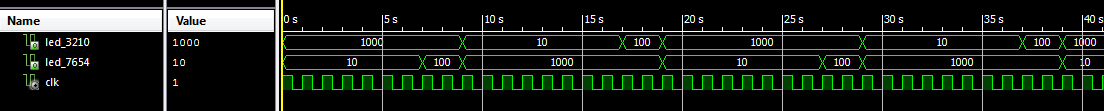
\includegraphics[width=1.0\textwidth]{files/tp3_2/simu_noreset.png}
   \caption{Simulation sans reset}
\end{figure}

On constate le bon fonctionnement de notre programme. L'alternance de feu s'effectue de la manière souhaitée.

\subsection{Ajout d'une fonction reset}

On réfléchit maintenant à l'intégration du reset dans notre code. Nous choisissons de le faire de manière synchrone.
Poue cela on modifie le code ci-dessus en insérant \textbf{une structure if...elsif} plutôt qu'un simple \textbf{if} détecteur d'horloge.

\vhdl
\begin{lstlisting}
[...]
process(clk,reset)
  [...]
  begin
  if reset = '1' then
  	state := 0;
  	i:=0;
  	a1:=8;
  	a2:=2;
  elsif (clk'event and clk='1') then
  		case state is
  		when 0 =>
  		  [...]
\end{lstlisting}

\begin{figure}[!h]
   \centering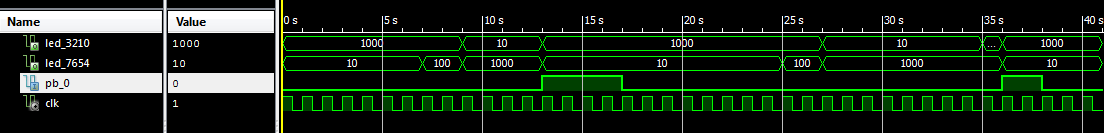
\includegraphics[width=1.0\textwidth]{files/tp3_2/simu_reset.png}
   \caption{Simulation avec reset}
\end{figure}

On simule notre reset : on constate bien que lorsque le reset est activé, notre signalisation est remise à son état initial (état 0) et maintenue dans cet état tant que le bouton est enfoncé.

\section{Exercice 3. Prise en compte d’un capteur de voiture.}
\subsection{Spécifications}
Par rapport à l'exercice précédent, nous avons rajouté deux états intermédiaires d'attente de véhicule.
\begin{itemize}
  \item État 0 : Les feux de l'axe 1 sont au rouge, ceux de l'axe 2 au vert. Rien ne se passe et on attend la détection d'un véhicule sur l'axe 1.
  \item État 1 : Un véhicule est détecté sur l'axe 1. On laisse les feux dans le même état pendant 8 secondes
  \item État 2 : Les feux de l'axe 1 sont au rouge, ceux de l'axe 2 au orange
  \item État 3 : Les feux de l'axe 1 sont au vert, ceux de l'axe 2 au rouge. Rien ne se passe et on attend la détection d'un véhicule sur l'axe 2.
  \item État 4 : Un véhicule est détecté sur l'axe 1. On laisse les feux dans le même état pendant 8 secondes
  \item État 5 : Les feux de l'axe 1 sont au vert, ceux de l'axe 2 au orange
\end{itemize}

\subsection{VHDL}

On propose le code VHDL suivant :

\vhdl
\begin{lstlisting}
entity circu is
	 port(LED_3210, LED_7654 : out integer range 0 to 15;
			PB_0, PB_2, PB_3, Clk100MHz : in bit);
end circu;

architecture Behavioral of circu is
	alias reset is PB_0;      -- alias pour le signal de réinitialisation
	alias detect1 is PB_2; -- alias pour la détection axe 1
	alias detect2 is PB_3; -- alias pour la détection axe 2
	signal clk : bit;
	
	component blinker port(Clk100MHz,PB_0 : in bit; LED_0 : out bit);
	end component blinker;

	begin
	C1 : blinker port map(Clk100MHz,PB_0,clk);
	
	process(clk,reset)
		variable state : integer range 0 to 5 := 0;
		variable i : integer range 0 to 7 := 0;
		variable a1 : integer range 0 to 16 := 8;
		variable a2 : integer range 0 to 16 := 2;
	begin
	if(clk'event and clk='1') then
		case state is
			when 0=> --Attente de détection sur l'axe 1
				if(detect1='1')then
					state:=1;
					a1:=8;
					a2:=2;
					i:=1;
				end if;
			when 1 => --On lance le temps de 8s de feu vert et on passe à l'orange
				if(i/=7) then
					i:=i+1;
				else
					state:=2;
					a1:=8;
					a2:=4;
					i:=0;
				end if;
			when 2 => --On attend 2s à l'orange puis on passe au rouge
				if(i/=1) then
					i:=i+1;
				else
					state:=3;
					a1:=2;
					a2:=8;
					i:=0;
				end if;
			when 3=> -- Attente de détection sur l'axe 2
				if(detect2='1')then
					state:=4;
					a1:=2;
					a2:=8;
					i:=1;
				end if;
			when 4 =>
				if(i/=7) then
					i:=i+1;
				else
					state:=5;
					a1:=4;
					a2:=8;
					i:=0;
				end if;
			when 5 =>
				if(i/=1) then
					i:=i+1;
				else
					state:=0;
					a1:=8;
					a2:=2;
					i:=0;
				end if;
			end case;
	end if;
	LED_3210<=a1;
	LED_7654<=a2;
	end process;
end Behavioral;
\end{lstlisting}

\subsection{Simulations}

On simule tout d'abord sans effectuer de reset :

\begin{figure}[!h]
   \centering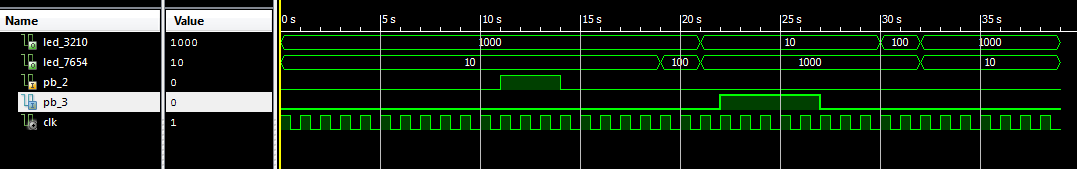
\includegraphics[width=1.0\textwidth]{files/tp3_3/simu_noreset.png}
   \caption{Simulation sans reset}
\end{figure}

On constate le bon fonctionnement de notre programme. Il y a bien une attente de détection sur un axe pour changer l'état de la signalisation, après les 8 secondes de feu vert prévues.

\medskip

On réfléchit maintenant à l'intégration du reset dans notre code. Nous choisissons de le faire de manière \textbf{synchrone} car plus sûr et plus simple. Pour cela on modifie le code ci-dessus en insérant \textbf{une structure if...elsif} plutôt qu'un simple \textbf{if} détecteur d'horloge.

\vhdl
\begin{lstlisting}
	[...]
	begin	
	if reset = '1' then -- Reset synchrone
		state := 0;
		i:=0;
		a1:=8;
		a2:=2;
	elsif(clk'event and clk='1') then
		case state is
			when 0=> -- Attente de détection sur l'axe 1
			[...]
\end{lstlisting}

On simule avec reset : 

\begin{figure}[!h]
   \centering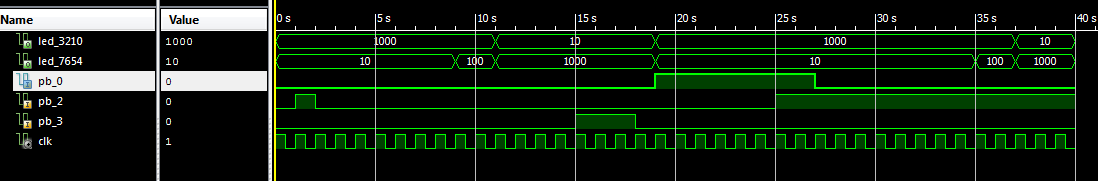
\includegraphics[width=1.0\textwidth]{files/tp3_3/simu_reset.png}
   \caption{Simulation avec reset}
\end{figure}

On constate le bon fonctionnement du signal de reset.